\chapter[Introdução]{Introdução}
O presente relatório trata de um projeto que visa auxiliar o condutor a realizar
 ultrapassagens em rodovias simples, de mão dupla, com segurança, a fim de evitar
 que motoristas tomem a decisão de fazer manobras arriscadas de ultrapassagem,
baseados apenas na própria experiência ou no bom senso.

Dentre os acidentes automotivos, os que possuem o maior número de vítimas fatais
são do tipo colisão frontal. De 2010 a 2014 quase metade dos acidentes com
fatalidades em rodovias federais, um total de 48,3\%, foram fruto desse tipo
de colisão e de atropelamentos. É um tipo de acidente que embora possua baixa
ocorrência é extremamente violento \cite{ipea}.

Essas informações recebem comprovação nos relatórios do \cite{ipea}, informando
que colisões frontais representam 4\% de todos os acidentes embora possua uma
parcela 24,6\% do total de mortes. 81,75\% dos acidentes desse tipo ocorreram
em pistas simples com tráfego nos dois sentidos e o principal motivo apontado
seria: ultrapassagem indevida, ultrapassagem de veículos lentos ou em
congestionamento e falta de visibilidade. \cite{fatoresCondicionantesGravidade}

Em outro relatório do \cite{ipea} curiosamente mantém a mesma porcentagem
apresentada no relatório recente de 2008 e pode ser acompanhado na Figura \ref{fig:visibilidade}.
\cite{custos_acidentes_transito}

\begin{figure}[h]
  \centering
  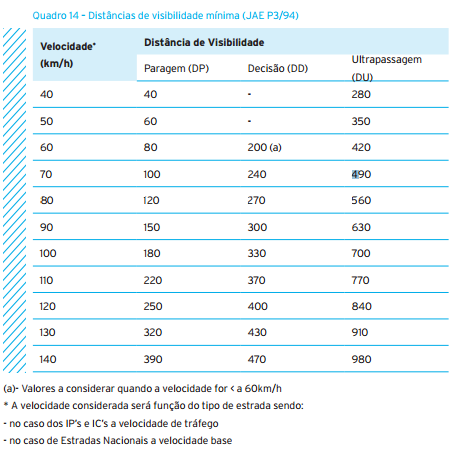
\includegraphics[width=400px, scale=1]{figuras/visibilidade}
  \caption{Tipo versus Gravidade dos acidentes em rodovias federais – 2004}
\label{fig:visibilidade}
\end{figure}

\begin{enumerate}
	\item Nome do projeto: Comunicação Interveicular para Alerta de Colisões em Rodovias
	\item Descrição do Projeto: Construção de um sistema que auxilie ultrapassagens com segurança
	\item Gerentes do Projeto: Tainara Costa e Renato Lucas
\end{enumerate}

\section{Tecnologia Existente}

SISTEMA TOYOTA Apenas dois carros da marca Toyota foram contemplados com o novo
sistema. São eles: RAV-4 hybrid e Lexus 2016. \cite{3comper} No RAV4, o sistema
anti colisão recebeu o nome de Toyota Safety Sense (TSS). O conjunto TSS permite
o cliente pode optar pelo TSSC e TSSP. O primeiro também traz sistema de mudança
de faixa e detector de farol alto. O segundo, destinado para veículos de médio
e grande porte, oferece ainda Radar Cruise Control e detector de pedestres. No
Lexus, a ferramenta é idêntica, porém recebeu um outro nome: Lexus Safety System
 + (LSS+). 5. Especificações do Sensor E FUNCIONAMENTO O funcionamento desse
sistema é apresentado em um vídeo disponibilizado pela Toyota. Nesse vídeo é
 possível perceber que o sistema foi criado para ser usado dentro e fora da cidade.
Trata-se um dispositivo que detecta possíveis casos de colisão. Tendo em vista a
situação de perigo, um alerta é disparado para avisar ao condutor da provável
colisão. Caso nenhuma iniciativa seja tomada para evitar a colisão, o próprio
sistema aciona os freios e reduz a velocidade do veículo para 30km/h. O vídeo
pode ser assistido pelo site: \cite{4comper}. É composto por uma câmera que
trabalha em parceria com um radar a laser. Entretanto, não é possível afirmar
modelo, marca ou exato funcionamento desses dispositivos.Entende-se,ao assistir
o vídeo, que tanto os sensores quanto o radar estão localizados na parte frontal
do veículo.

\begin{figure}[h]
  \centering
  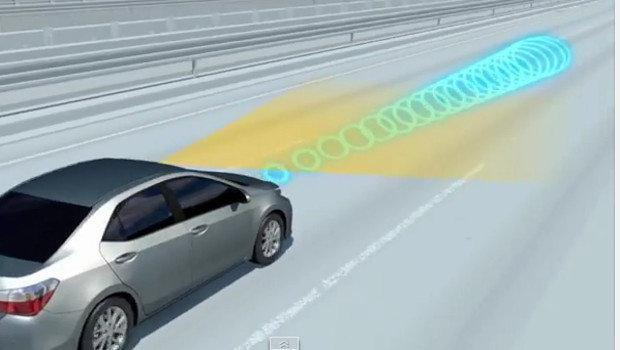
\includegraphics[width=400px, scale=1]{figuras/sinal_componentes}
  \caption{Revista Quatro Rodas}
\label{fig:sinal_componentes}
\end{figure}

Custo No RAV4 o SafetySense(TSS) será um opcional. Logo, o comprador deseja um
veículo que ofereça maior segurança, terá que pagar US\$30,00 a mais. No Lexus,
Safety System + (LSS+), o valor pago a mais será de US\$ 500,00. \cite{1comper}.

\section{Solução}

Com o auxílio dos sensores LIDAR e Radar para detectar a distância de outros
veículos; sensores de rotação, o indicador da seta do veículo e a câmera capaz
de detectar mudanças de faixa, para identificar intenção de ultrapassagem; um
sistema de comunicação que utiliza da tecnologia dos transponders; Um GPS para
auxiliar na identificação da posição do veículo, o sistema emitirá alertas de
colisão indicando quando é seguro ultrapassar um veículo. Este conjunto de
equipamentos, juntamente com os controladores/processadores detectarão os
veículos ao redor, realizarão os cálculos em tempo real para determina as
distâncias e velocidades, além da direção e sentido deles, a fim de auxiliar o
condutor na tomada de decisão da ultrapassagem ou alertá-lo caso esta não seja viável.

\section{Objetivo}
Espera-se que o projeto deste sistema seja capaz de auxiliar na construção e
comercialização desta tecnologia de prevenção de acidentes e que todos os veículos
contenham-na, a fim de que ela reduza os índices de colisões frontais nas rodovias
brasileiras.

\section{Metodologia}

\subsection{Aplicação do Scrum no CIAC}
Dentro de cada release, foram definidas várias sprints, cada uma com o timebox de
uma semana. O marco para término da sprint é segunda feira, onde as atividades
serão desenvolvidas até o dia anterior. Há um encontro presencial em todos os
dias de término da sprint, onde, são executadas as reuniões de Revisão da Sprint,
 Retrospectiva da Sprint e Planejamento da Sprint contendo todas as equipes do projeto.

O projeto é composto por cinco times Scrum, cada um com seu Scrum master. O
conjunto de Scrum masters é dirigido pelos dois Products Managers: Tainara e Renato.

 As demais equipes estão organizadas como a figura  \ref{fig:time} a seguir: Como pode ser visto
, cada time irá tratar de um propósito no trabalho ligado as cinco
engenharias. Cada um desses grupos tem atividades prórprias que remetem o seu escopo.

\begin{figure}[h]
  \centering
  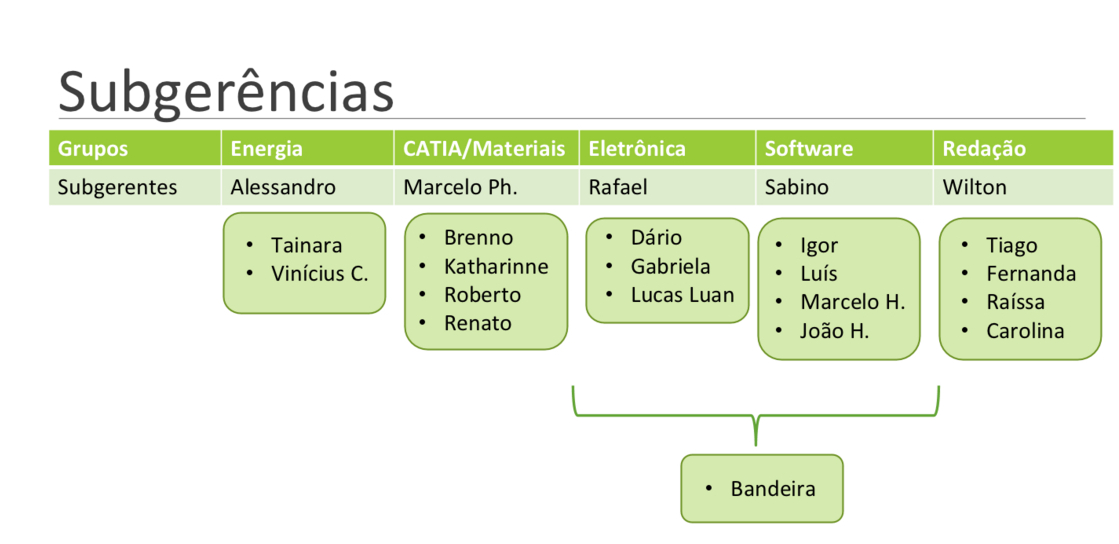
\includegraphics[width=400px, scale=1]{figuras/time}
  \caption{Divisão do Time Scrum}
\label{fig:time}
\end{figure}

A partir da primeira release, surgiu o grupo de redação, responsável por escrever
o relatório e formatá-lo nos padrões exigidos. Além disso, existe um scrum master
responsável por gerencias os times de eletrônica e software. Essa decisão foi
tomada, pois, há muita interação entre as equipes, assim, este é responsável por
fazer a ligação de ambas as partes que devem estar em sincronia.

O backlog do produto é gerenciado pelos Products Managers e dividido aos Scrum
Masters(Subgerente). Cada time de desenvolvimento trabalha a partir de um Sprint Backlog
destinado a cada subgerente naquela semana de desenvolvimento e validado no dia
da reunião de revisão da sprint.

\subsection{Ferramentas de Comunicação e Desenvolvimento}
\subsubsection{Slack}
A plataforma de comunicação em grupo Slack foi adotada pelo grupo como meio de comunicação principal.
Sendo centralizada nela as principais informações e debates relevantes ao escopo do projeto.

\begin{figure}[h]
  \centering
  
\includegraphics[width=300px, scale=0.5]{figuras/slack}
  \caption{Plataforma de Comunicação Slack}
  \label{table:slack}
\end{figure}


\subsection{WhatsApp}
O WhatsApp foi escolhido como meio de comunicação secundário enquanto todos os integrantes do grupo
não migrassem para a plataforma principal. Lá se concentraram os esforços de contato inicial para reunir
todos os integrantes da equipe.

\begin{figure}[h]
  \centering
  
\includegraphics[width=300px, scale=0.5]{figuras/wpp}
  \caption{Plataforma de Comunicação WhatsApp}
  \label{table:wpp}
\end{figure}


\subsubsection{Trello}
O Trello foi escolhido como meio de gerenciamento de projetos, definindo grupos e
frentes de trabalho. Cada um com a sua devida atividade.

\begin{figure}[h]
  \centering
  
\includegraphics[width=300px, scale=0.5]{figuras/trello1}
  \caption{Plataforma de Gerência de Projetos}
  \label{table:trello1}
\end{figure}


\subsection{Google Drive}
O Google Drive foi escolhido como ferramenta para armazenamento dos arquivos e artefatos importantes para a
equipe. As entregas parciais de documentos e pesquisas dos integrantes foram todas centralizada nesta plataforma
para efeitos de backup de documentos.
\begin{figure}[h]
  \centering
  
\includegraphics[width=300px, scale=0.5]{figuras/google_drive-logo}
  \caption{Ferramenta de Armazenamento Google Drive}
  \label{table:google_drive-logo}
\end{figure}
\subsubsection{Latex}
O \LaTeX\ foi a ferramenta designada para a estruturação e escrita do relatório.
\begin{figure}[h]
  \centering
  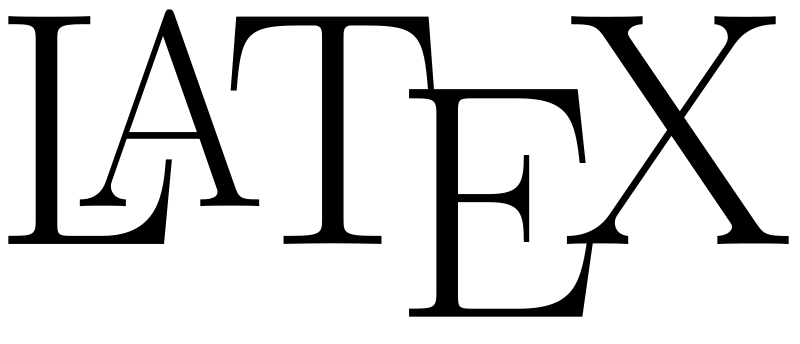
\includegraphics[width=200px, scale=0.5]{figuras/latex_logo}
  \caption{Ferramenta de Marcação de Texto LaTeX}
  \label{table:latex_logo}
\end{figure}
\subsubsection{Git}
Como ferramenta de versionamento utilizou-se o Git para gerenciar as mudanças e atualizações do conteúdo do slide
por todos os membros da equipe. Essa ferramenta foi escolhida pelo grupo para evitar diferenças e centralização do
conteúdo do relatório. Pois o mesmo foi armazenado em um repositório online para acesso de todos os membros do projeto.
\begin{figure}[h]
  \centering
  
\includegraphics[width=200px, scale=0.5]{figuras/git}
  \caption{Ferramenta de Versionamento GitHub}
  \label{table:git}
\end{figure}
\subsubsection{Editores de Texto}
\label{sub:Editores de Texto}
Para editar o textos compilados em LaTeX foram utilizados dois editores de texto diferentes:
\begin{itemize}
  \item Sublime text Editor
  \item Atom text Editor
\end{itemize}

\begin{figure}[h]
  \centering
  
\includegraphics[width=200px, scale=0.5]{figuras/sublime}
  \caption{Editor de Texto Sublime}
  \label{table:sublime}
\end{figure}
\begin{figure}[h]
  \centering
  
\includegraphics[width=200px, scale=0.5]{figuras/atom}
  \caption{Editor de Texto Atom}
  \label{table:atom}
\end{figure}

\section{Cenário de implementação}
\subsection{Estudo de locais}
A BR 262 é uma rodovia transversal brasileira que liga os Estados do Espírito
Santo, Minas Gerais, São Paulo e Mato grosso do Sul. Tem início em Vitória (ES) e
passa por cidades importantes como Manhuaçu, Belo Horizonte, Araxá, Uberaba, Três
Lagoas e Campo Grande. Percorre 999,8 Km no estado de Minas Gerais cortando-o de
leste a oeste. Em 2009 apresentou um elevado número de acidentes. Ao todo foram
registrados 9.614 acidentes em que 280 pessoas morreram. Somente no percurso entre
Belo Horizonte e Governador Valadares houveram 2.975 acidentes, no qual 2.159
ficaram feridas e 138 vieram a óbito. Atualmente já possui trechos duplicados,
mas ainda conta com muitos trechos de mão simples.
\cite{wikipedia}

\begin{figure}[h]
  \centering
  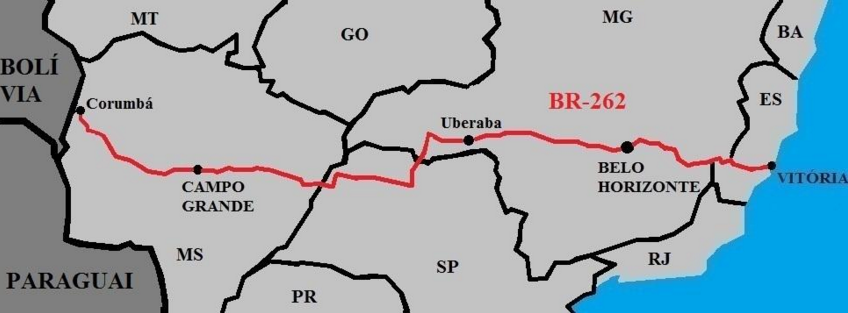
\includegraphics[width=400px, scale=0.5]{figuras/mapa}
  \caption{Rota BR 262}
  \label{table:mapa}
\end{figure}

\subsection{Justificativa}
Em 2014 o Estado de Minas Gerais foi o que apresentou o maior número de acidentes
e mortos em rodovias, seguido por Paraná, Santa Catarina, São Paulo e Rio de
Janeiro. Essas regiões contabilizam a maior parte da riqueza do país, sendo assim
há maior geração de viagens e quantidade de veículos motorizados, fatores que
interferem no número de tráfego e acidentes. Seguem alguns dados da tabela \ref{table:tabelaacidentes}


\begin{figure}[h]
  \centering
  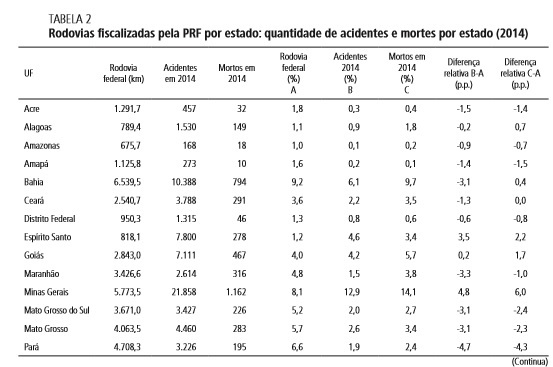
\includegraphics[width=400px, scale=0.5]{figuras/tabelaacidentes}
  \caption{Quantidade de acidentes e mortes por estado}
  \label{table:tabelaacidentes}
\end{figure}

Considerando-se os tipos de acidente, verifica-se que a colisão frontal foi responsável
por 33,7\% das mortes. Nos acidentes desse tipo morreram 40,4 pessoas a cada 100
acidentes. 89,71\% das colisões frontais ocorreram em pistas simples, ocasionando
93,91\% dos mortos nesse tipo de acidente. A maior causa dos acidentes é a falta
de atenção do motorista.

Mesmo não sendo a rodovia mais perigosa e com maior número de acidentes, a BR 262
é considerada uma rodovia perigosa pois apresenta muitos trechos simples de mão
dupla, além de algumas deficiências como falta de sinalização e condições ruins
de tráfego, o que favorece o implemento do sistema anticolisão veicular. A título
de curiosidade, a BR 381( Fernão Dias) é a que mais possui acidentes, porém não
são colisões frontais já que inteira duplicada. O trecho entre os Km 490 a 500,
na altura de Betim é o que apresenta maior número de acidentes.

\begin{figure}[h]
  \centering
  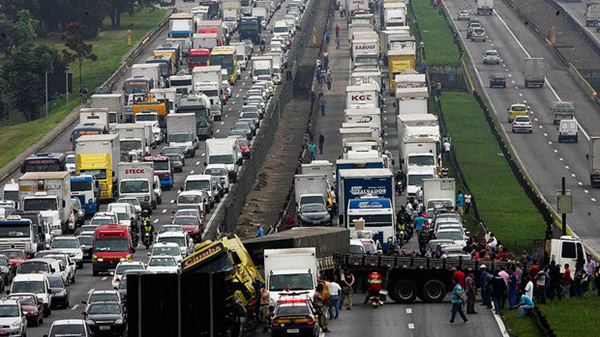
\includegraphics[width=400px, scale=0.5]{figuras/br381}
  \caption{BR 381 (Fernão Dias)}
  \label{table:br381}
\end{figure}

\subsection{Veículos envolvidos em acidentes}
Em 2013, a PRF registrou um número de 186.474 acidentes nas rodovias federais
brasileiras. Em 2014, tínhamos uma frota de 81,3 milhões de veículos.

Os automóveis apresentam o maior percentual de envolvimento nos acidentes de
trânsito nas rodovias e também mortes entre todos os modais de transporte, em
função do maior número da frota circulante. O gráfico a seguir nos traz números
exatos

\begin{figure}[h]
  \centering
  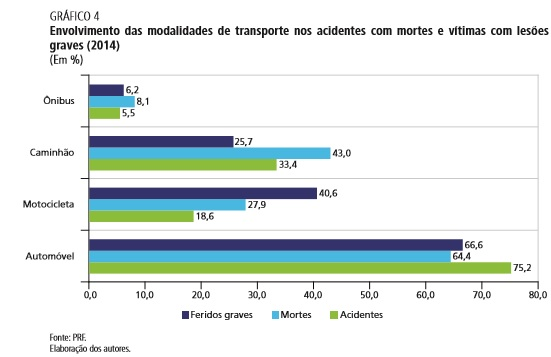
\includegraphics[width=400px, scale=0.5]{figuras/niveisacidente}
  \caption{Envolvimento das Modalidades de Transporte \cite{ipea3}}
  \label{table:niveisacidente}
\end{figure}

Desde 2007 a PRF vem fazendo levantamento de dados sobre quais são os veículos
que mais se envolvem em acidentes. Em primeiro lugar temos o Volkswagen Gol, que
esteve presente em 14.125 acidentes. Em segundo lugar vem o Fiat Uno, envolvido
em 8200 acidentes, seguido pelo Fiat Palio, com registro de 7.041 acidentes. Em
quarto lugar vem o Chevrolet Celta, participando de 5.931 acidentes. Em quinto
lugar temos a Honda CG 150, envolvida em 5.784 acidentes.

Sendo assim, o sistema anticolisão veicular será implantado no Volkswagen Gol,
afim de ilustrar nosso cenário na BR 262.
